\documentclass{scrartcl}

% neccesarry for style
\usepackage[english]{babel}
\usepackage[utf8]{inputenc}
\usepackage[T1]{fontenc}
\usepackage{lmodern}

% tools for text
\usepackage{csquotes}
\usepackage{url}
\usepackage{hyperref}

% graphics
\usepackage{graphicx}
\usepackage{xcolor}
\usepackage{tikz}

% maths
\usepackage{amsmath,amssymb,amstext,amsthm}

% programming
\usepackage{listings}

\usepackage{wasysym} %lightning

\input{required/settings.tex}
\input{required/commands.tex}

\renewcommand{\labelenumi}{\alph{enumi})}
\begin{document}
	\begin{center}
		\LARGE
		Information Integration -- Exercise 5 -- Gabriel Glaser
	\end{center}
	
	\section*{Task 1: Schema Mapping}
	\begin{center}
		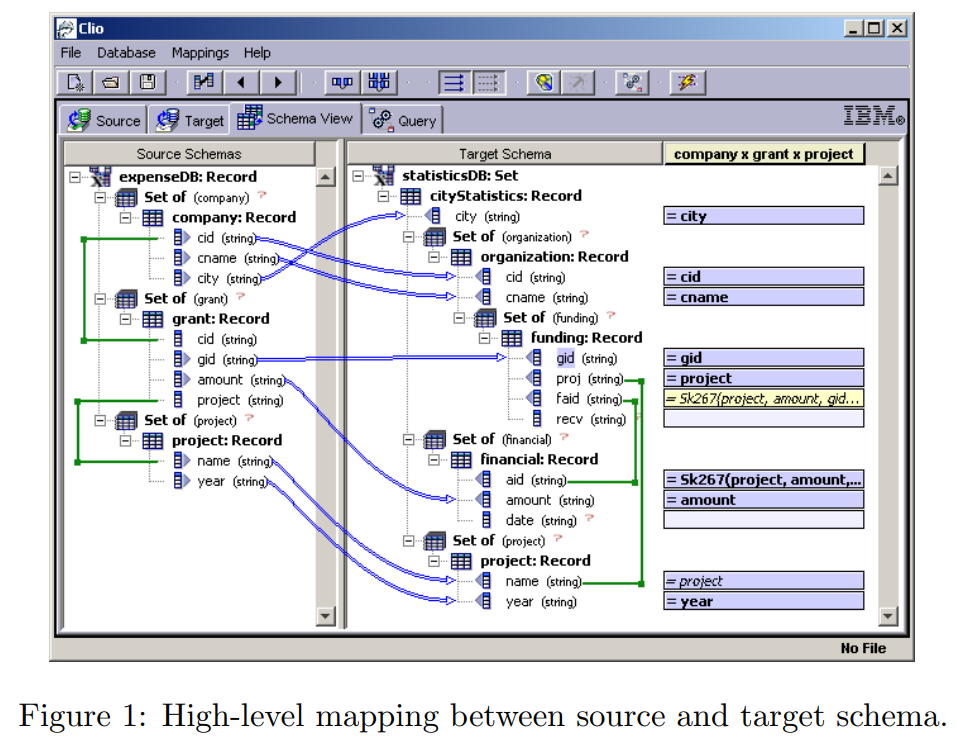
\includegraphics[width=0.9\textwidth]{figures/task1_image.PNG}
	\end{center}
	\begin{center}
		\fbox{
		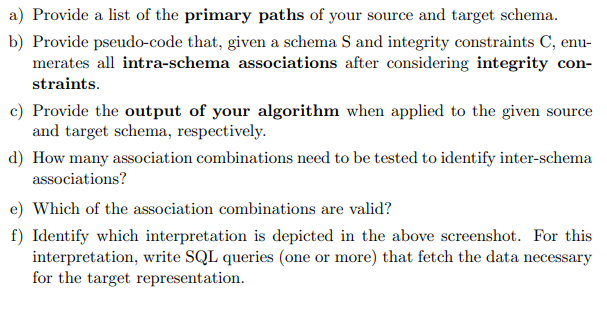
\includegraphics[width=0.9\textwidth]{figures/task1_description.PNG}}
	\end{center}
	\begin{enumerate}
		\item \textit{Primary paths of source schema}:
		\begin{itemize}
			\item company
			\item grant
			\item project
		\end{itemize}
		
		\textit{Primary paths of target schema}:
		\begin{itemize}
			\item cityStatistics
			\item cityStatistics, organization
			\item cityStatistics, organization, funding
			\item cityStatistics, financial
			\item cityStatistics, project
		\end{itemize}
		
		\item\phantom{phantom}
		\begin{center}
			\fbox{
				\begin{tabular}{l}
					\textbf{function} enumerateIntraSchemaAssociationsWithIC(S, C):\\
						\hspace{0.5cm}List<List<Attribute>{}> primaryPaths = \textit{getPrimaryPaths}(S);\\
						\hspace{0.5cm}List<List<Attribute>{}> primaryPathsWithIC = [ ];\\
						\hspace{0.5cm}\textbf{for} (List<Attribute> primaryPath \textbf{in} primaryPath):\\
							\hspace{1cm}List<Attribute> primaryPathWithIC = [ ];\\
							\hspace{1cm}\textbf{for} (0 $\leq$ i $<$ \textit{length}(primaryPath)):\\
								\hspace{1.5cm}Attribute attribute = primaryPath[i];\\
								\hspace{1.5cm}primaryPathWithIC.\textit{append}(attribute);\\
								\hspace{1.5cm}Set<Attribute> foreignKeyAttributes = \textit{getForeignKeys}(attribute, C);\\
								\hspace{1.5cm}primaryPathWithIC.\textit{appendAll}(foreignKeyAttributes);\\
							\hspace{1cm}primaryPathsWithIC.\textit{append}(primaryPathWithIC);\\
						\hspace{0.5cm}\textbf{return} primaryPathsWithIC;
				\end{tabular}
			}\\
			\vspace{0.5cm}
			\fbox{
				\begin{tabular}{l}
					\textbf{function} getPrimaryPaths(S):\\
					\hspace{0.5cm}\textbf{if} \textit{isRelational}(S):\\
					\hspace{1cm}\textbf{return} \textit{getAllTables}(S);\\
					\hspace{0.5cm}\textbf{else}:\\
					\hspace{1cm}Tree<Attribute> tree = \textit{recursivalyDescend}(S);\\
					\hspace{1cm}\textbf{return} \textit{getAllSubPathsToLeafs}(tree);\\
				\end{tabular}
			}\\
		\end{center}
		
		\item \textit{Output of algorithm applied on source schema}:
		\begin{itemize}
			\item company
			\item grant, \textbf{company}, \textbf{project}
			\item project
		\end{itemize}
		
		\textit{Output of algorithm applied on target schema}:
		\begin{itemize}
			\item cityStatistics
			\item cityStatistics, organization
			\item cityStatistics, organization, funding, \textbf{financial}, \textbf{project}
			\item cityStatistics, financial
			\item cityStatistics, project
		\end{itemize}
		
		\item Three associations combinations for source schema, Five associations for target schema, i.e., $3\cdot5=15$ tests.
		
		\item Valid association combinations:
		\begin{itemize}
			\item company $\to$ cityStatistics, organization
			\item grant, company, project $\to$ cityStatistics, organization, funding, financial, project
			\item project $\to$ cityStatistics, project
		\end{itemize}
		
		\item Interpretation depicted in screenshot:
		\begin{itemize}
			\item For each \textbf{company} element, create a \textbf{cityStatistics.organization} element with respective \textbf{cid} and \textbf{cname}.
			Group the created elements under \textbf{company.city} as \textbf{cityStatistics.city}.
			
			\item For each \textbf{grant} element, add a \textbf{funding} element to the set of the \textbf{cityStatistics.organization} with same \textbf{cid}.
			The \textbf{gid} is given, but \textbf{faid} and \textbf{recv} have to be invented (e.g., with skolem function), because there are no key-constraints or high-level mappings.
			
			To finish the funding element, use the \textbf{project.name} value for \textbf{funding.proj}, because \textbf{project} of source and \textbf{proj} of target are involved in a key constraint of value which are connected with a high-level mapping.
			
			Finally, create a \textbf{financial} entry (for the \textbf{cityStatistics} in which the a \textbf{cityStatistics.organization} with respective \textbf{cid} occurs) with the given \textbf{amount} and invented \textbf{date} and previously invented \textbf{faid} as \textbf{aid}.
			
			\item For each source \textbf{project} element (with \textbf{name} and \textbf{year}) create \textbf{cityStatistics.project} element for each \textbf{cityStatistics} for which there exists a \textbf{funding} with \textbf{project.name} = \textbf{cityStatistics.organization.funding.proj}.
		\end{itemize}
		
		SQL-Queries:
		\begin{center}
			\fbox{
				\begin{tabular}{l}
					\textbf{CREATE} \textbf{VIEW} GrantData \textbf{AS}\\
					\hspace{0.5cm}\textbf{SELECT} * \textbf{FROM} grant\\
					\hspace{1cm}\textbf{INNER} \textbf{JOIN} company \textbf{ON} grant.cid=company.cid\\
					\hspace{1cm}\textbf{INNER} \textbf{JOIN} project \textbf{ON} grant.project=project.name;
				\end{tabular}
			}
		\end{center}
		Get data of remaining companies which don't have a grant:
		\begin{center}
			\fbox{
				\begin{tabular}{l}
					\textbf{CREATE} \textbf{VIEW} CompanyData \textbf{AS}\\
					\hspace{0.5cm}\textbf{SELECT} * \textbf{FROM} company\\
					\hspace{1cm}\textbf{WHERE} \textbf{NOT} \textbf{EXISTS} (\textbf{SELECT} grant.cid \textbf{FROM} grant\\
					\hspace{1.5cm}\textbf{WHERE} company.cid=grant.cid);\\
				\end{tabular}
			}
		\end{center}
		Get data of projects and join with company such that the projects can be listed under the right \textbf{cityStatistics.city}.
		(A project can be listed under multiple)
		\begin{center}
			\fbox{
				\begin{tabular}{l}
					\textbf{CREATE} \textbf{VIEW} ProjectData \textbf{AS}\\
					\hspace{0.5cm}\textbf{SELECT} * \textbf{FROM} project\\
					\hspace{0.5cm}\textbf{INNER} \textbf{JOIN} company \textbf{WHERE} \textbf{EXISTS}\\
					\hspace{1cm}(\textbf{SELECT} * \textbf{FROM} grant \textbf{WHERE} grant.cid = company.cid\\
					\hspace{1cm}\textbf{AND} grant.project=project.name);
				\end{tabular}
			}
		\end{center}
	\end{enumerate}
\end{document}
